Technologies for verification and debugging have made significant strides in the context of general systems software. An investment in such technologies to make them applicable for High Performance Computing (HPC) could lead to substantial improvements in the productivity and sustainability of HPC software development. Such improvements will be essential to fully exploit new exascale computer architectures.
\ignore{------
The technology for verification and debugging in support of correctness has advanced to the point that there is a basis for confidence in success of investment in the application and advancement of such tools 
%--for correctness 
in High Performance Computing (HPC).  With such investment, the field of computational science will benefit from substantial improvements in the ability to exploit new exascale computer architectures, and from substantial improvements in productivity and sustainability of HPC software development.
-----}  Without such investment, there is the possibility of a substantial crisis in our ability to advance the field of HPC, as the complexity of our architectures, algorithms, and applications is moving beyond the ability of our developers.  As HPC is of strategic importance to our nation, forming the bedrock of its scientific and technological capabilities, such investment is highly warranted.

\subsection{Reasons for the correctness crisis}

While the general correctness problem in computer science is well
researched, specific reasons that cause HPC-specific correctness
methods to turn into an urgent priority include the following (see
Figure~\ref{fig:overview-challenges}
for an overview).

\paragraph{Growing heterogeneity:}

  Given the widening disparities between CPU, memory, and I/O speeds,
  computations will be supported by a heterogeneous architectures that include CPUs, GPUs, and special-purpose accelerators~\cite{hwu-heterogeneity}.
  %
 Even today,
  programs in this space exist around a patchwork of semantic
  abstractions that are poorly understood individually, and
  whose emergent behavior is poorly understood.

\paragraph{Massive scale:}

  Attaining exascale will require proper coordination and synchronization
  across many tasks, threads, and processes~\cite{exascale-computing-project}.
  Disciplines that guide programming in this space do not exist, nor do testing methods that unearth defects in this space.
Left unchecked, this will lead to deployed systems that yield untrustable results or
crash during long-running simulations. 
Fixing the root cause of bugs in these
settings will incur huge latencies during which science
domain
experts may sit idle or be unproductively engaged with
debugging. These costs are known to be already very high (see the sidebars for some concrete examples of costly field bugs in HPC).
\ignore{----
but seldom highlighted in summary reports of HPC projects.
----}


% ilaguna
\begin{figure}
\centering
\begin{adjustbox}{width=1.15\textwidth,center}
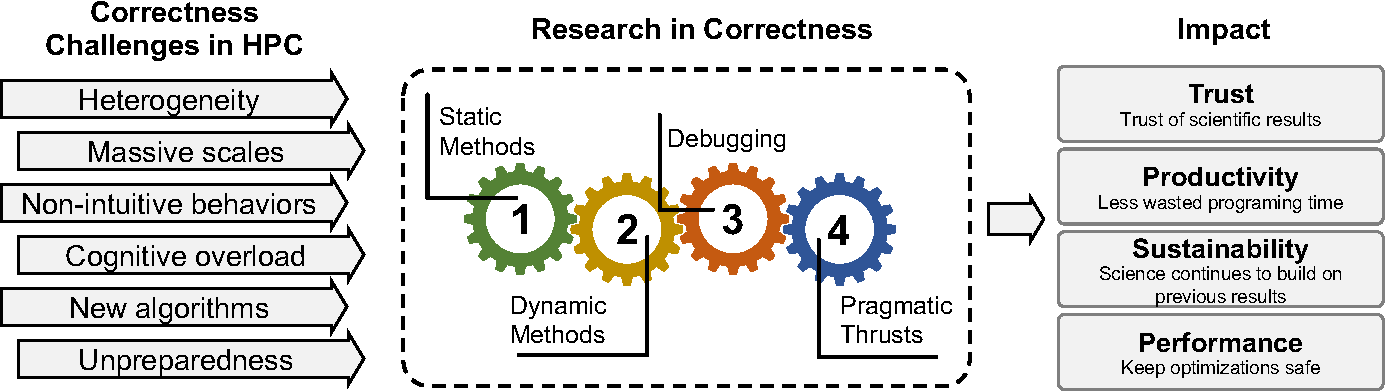
\includegraphics[width=0.99\textwidth]{figures/overview_diagram.pdf}
\end{adjustbox}
\caption{Overview of the existing challenges in correctness for HPC and the research areas that need extensions to address these challenges.}
\label{fig:overview-challenges}
\end{figure}


\paragraph{Non-intuitive behaviors:}
 The push toward significant energy savings will lead to the use of
  reduced floating-point arithmetic, delayed state updates across weak
  memory consistency models, non-determinism caused by dynamic
  voltage/frequency scaling, fault recovery steps and inherent
  application non-determinism.  It is impossible to employ ad hoc
  debugging methods in these situations.


\paragraph{Cognitive overload:}
The manner in which people write as well as
configure full applications is
evolving in a direction where human reasoning about correctness is impractical.
  For example, the NWChemEx computational chemistry code is bringing together SPMD and task parallelism, multiple programming models and runtime interfaces, code generation, and dynamic and adaptive selection of execution configurations. 
In these settings, manually reasoning about correctness of the application, or even an individual execution, has gone beyond the scope of the individual developers;
the need to bring in more automated and/or
formal ways has become quite apparent.



\paragraph{New scalable algorithms:}
New algorithms for numerical computing offer the potential for major improvements in the asymptotic requirements for computation~\cite{ascac-2017}.  Kernel-independent and generalized Fast Multipole Methods (FMM) enable matrix vector multiply to be achieved in $O(N)$ time.  Support preconditioner methods will enable sparse systems of equations to be solved in near-linear time.  Randomized linear algebra and compressive methods will enable systems to be simulated in sampled or compressed form.  Such algorithms will bring complex new execution patterns and complex tradeoffs between precision, probability, and time.  The ability to exploit these algorithms will require tools to facilitate reasoning about the correctness of their application and implementation.

  %
%--Sriram
\begin{WrapText}
\footnotesize
{\large \textbf{Undoing an optimization leads to a difficult bug}} \\

Tensor contraction expressions in Coupled Cluster methods involve products of multiple anti-symmetric tensors. In NWChem, these expressions are computed as a chain of pairwise tensor contraction to minimize operation count. An effort to reoptimize these contractions in the new generation of tensor contraction engine (TCE) by undoing the chaining and reoptimizing the contraction sequence in the existing TCE led to incorrect results. Isolating the source of the error was a manual process: transforming subsets of the contractions and checking for differences. After months of effort, it was found that, depending on the chaining, an additional coefficient needed to be introduced in a key intermediate step, referred to as symmetrization. Explicit specification of the optimization rules and checking whether or not the transformations satisfy the rules could have identified this bug quickly.
\end{WrapText}



  
\paragraph{Community unpreparedness:} \mbox{ }\\
  Compared to sequential programming abstractions that are more familiar
  to an application scientist, future HPC systems will involve a large
 slew of semantic abstractions (and relatively
 newer abstractions such as tasking)
 whose correct and efficient usage are
  not first nature to the broad application development community.
 
Ways to insulate application developers through
domain-specific languages (DSL) are badly needed; yet,
progress is lacking in this direction.
A related but severe problem is that
HPC application developers do not have the mindset
(or the necessary common repositories) for sharing
best practices (including
  sharing information on bugs and bug-fixes).
  This lack will hamper 
the transitioning of new verification research results into practice.
  

  
  \ignore{==> Ganesh addressed this above:
\todo[inline]{Should we include two more reasons: (1) use of DSLs, 
(2) use of task-based programing models?}
<==}





\subsection{What is in scope, what is not}

%To delineate the concerns addressed
%in this report, we outline issues within the scope of this report followed by a sampling of issues considered out-of-scope.



\paragraph{Current issues in scope:}
%
Any defect a programmer can correct by modifying and/or repairing
existing programs and/or their support runtime logic are well within the scope of this report.
These include
the classic sequential program bugs, errors relating to concurrency
(e.g., race conditions, incorrect programming under weak memory
models), and numerics (e.g., errors in realizing the numerical
algorithm using finite-precision floating-point numbers).  Defects that may
manifest only when a code is scaled up and not  during
lower-scale testing are also in scope.

We also consider defects that can be eliminated by disciplined code
 transformations from higher-level, or can be eliminated through
 better composition and software engineering practices.  Defect
 prevention methods that can be incorporated into best practices,
 pedagogy, mineable bug repositories, expert tutorials, and IDEs that
 can prevent or issue warnings about possible bugs are also of great
 importance, and are well within scope.

    % by ilaguna
  %--
  \begin{WrapText}
\footnotesize
{\large \textbf{A Hard-To-Debug Large-Scale Error}}\\
A bug in ddcMD, a parallel molecular-dynamic code, manifested as an
intermittent hang when run at large scale on BlueGene/L at LLNL.
It took a significant amount of person hours and debugging effort 
to find the root cause: a message race in which a process could 
hang waiting for a message that was intercepted by 
another process. More specifically, the hang occurred when 
two independent instances of a user-level I/O layer
were simultaneously processing two separate sets of buffers---an infrequent pattern that occurred when a small data set 
was written immediately after a large data set. Due to the 
semantics of MPI send/recv operations and the use of fixed tags, 
messages from a small set could be confused for those for a 
large set and vice versa, thus triggering the hang. 
Later, after the bug was fixed by the programmer, the bug was 
used in a blind study, in which researchers developed a tool 
to isolate this class of bugs without having details of the error 
(more in~\cite{PACTLaguna:2012}). This shows that documenting 
bug cases can be useful in developing and testing advanced 
correctness tool.
\end{WrapText}


  %--
  

When defining the correctness of HPC programs, it is important to keep in mind that the behavior of a user-written program is heavily influenced by the
behaviors of the underlying libraries.
%
Not only are the sequential (e.g., numerical and C/Fortran) libraries important, the behavior of communication and runtime libraries (e.g., MPI and OpenMP) directly impact how a user program executes and whether it even makes forward progress.

In this context, it is important to detect
and eliminate
erroneous arguments supplied to library functions
that may cause a program crash. 
For example, MPI calls must adhere to conventions pertinent to
the source language (Fortran or C).
%
However, resource aspects of the runtime and communication libraries are a whole different matter.
%
%
For example, it is possible to write a user program that may be perfectly correct as far as the users' mental model of an ``idealized MPI library'' goes, but unfortunately a given MPI library may be unable to park all the asynchronous sends that the user program has issued.
%
Such user programs can either deadlock or crash an MPI library.


Most libraries are
underspecified, and their implementations often do not come with strong
guarantees, such as about the amount of resources provided (e.g., amount of
buffering) or whether forward progress or a response within a
deadline is guaranteed. 
%
These issues are clearly also important, but must be relegated to a longer-term pursuit that involves cooperation from library and runtime designers.




In the same vein,
the inability to control the evolving semantics of libraries and
programming languages must be kept in mind, requiring cooperation
among participant communities.   For instance, if a library
guarantees a certain order of accuracy for its results (e.g., ``9
digits of accuracy'') for specific platforms, we may not be prepared
to detect the violation of such contracts by another library
on a newer platform to which the code is ported.

 % by ilaguna
%--
\begin{WrapTextLeft}
\footnotesize
{\large \textbf{When More Than \textit{print} Debugging Is Needed}}\\
A scientist experienced hangs in a laser-plasma interaction code 
(named PF3D) when scaling it to 524,288 MPI processes on 
LLNL’s Sequoia BlueGene/Q system. The scientist spent months trying 
to debug the problem through print statements to no avail. 
Moreover, the scientist was unable to reproduce the hang at 
smaller scales where fully featured, heavyweight debuggers 
would be more plausible. Using STAT (Stack Trace Analysis Tool), 
the scientist was able to debug the problem, a race condition 
between two distinct but overlapping communication code regions. 
The bug was the result of the application migrating from one version to another more scalable but incompatible one. During migration, the application ran 
through a compatibility layer that introduced the race condition 
and ultimately caused the timing- and scale-dependent hangs 
(more in~\cite{CACM:Debugging}). This case shows that, although 
print debugging can be a useful debugging method, 
the HPC community can benefit from advanced correctness 
methods and tools to isolate bugs that otherwise can consume 
months of effort and millions of CPU hours to fix.

\end{WrapTextLeft}
%--




\paragraph{Upcoming issues in scope during exascale:}
We also realize that
this report is being written in a timeframe where the underlying designs of exascale systems are experiencing significant disruptive changes.
%
In this era, hardware will often be poorly specified, particularly with regard to features related to
the memory model, concurrency and synchronization.  With exascale, new hardware features
for controlling voltage and frequency, are appearing, as well as advanced features for
task scheduling, communication, and synchronization. 
%
There will be heavy uses of heterogeneous types of memory (e.g., non-volatile, scratchpad spaces that do not provide cache coherence, etc.).
%
Consider the behavior
of an adaptive congestion algorithm~\cite{jiang2009indirect} in the communications fabric, which may 
affect or permute the ordering of delivery of messages. If such features are
not specified or are incorrectly specified to the runtime or MPI libraries, it will be impossible for any verification technology to guarantee correctness of the software running on it.  



The performance behavior of hardware is also moving into the arena
of correctness and even safety, where exascale hardware systems are likely to be
over-provisioned with transistors, so that not all 
parts of the system can be used simultaneously while still remaining below
the power and cooling limits of the facility, and within the limits for safe and correct operation of the machine.  This will impose requirements
on firmware, system software and applications to maintain resource usage.  

All these
issues clearly point to an even greater 
demand for formal specifications from the hardware
vendors on these behaviors and requirements.
It will also correspondingly demand that our formal verification
and debugging tools use these hardware level formal specifications in order to provide overall correctness guarantees.

   
  %--
% by ganesh
\begin{WrapText}
\footnotesize
{\large \textbf{Heterogeneity-caused arithmetic divergence results in deadlock}}\\
  In a recent project~\cite{xsede13-porting-bug},
an attempt to port some of the MPI processes to run on
Xeon-Phis while leaving others running on Xeons
caused a curious deadlock that took days to debug.
%
The root cause was the Xeon-Phis calculating the number of
messages to be sent (through an expression
$\lfloor p/c\rfloor $) differently from how the Xeons calculated
the number of messages to be received (also governed by $\lfloor p/c\rfloor$).
%
Unfortunately, the developers had not applied due precautions
to their compilation flags, resulting in $63$ messages 
being sent but only $62$ attempted to be received, which
then caused the deadlock.
%
This bug tells us that a 
combination of factors---processors
being different, floating-point 
roundoff differing
due to the inconsistent use of 
compiler optimization flags, and
the delicate MPI semantics allowing
the number of receives posted to exceed
the number of sends posted (but not
vice versa)---may  lead to bugs.
\end{WrapText}
     


 

\paragraph{The following issues are not directly within scope:} There are many issues that are important to keep in mind, but are best relegated to other pursuits that are better able to focus on them. 
%
We now mention a few examples of such issues (by no means exhaustive).
%
HPC programs may be brought down by
hardware logic errors in microprocessors, GPUs,
memory subsystems, and  buggy interconnect
protocol implementations.
%    
Soft errors may corrupt program behavior, but are not considered human-introduced 
defects.
%
Version control and security-related issues are again somewhat tangential.
%
Finally, the numerical algorithm itself can be incorrect.
%
For instance,
errors in the design of the numerical scheme to
approximate the idealized mathematics,
including incorrectly scheduled coarse/fine meshing, lack of
conditioning of the problems, etc.,
can be considered {\em algorithmic}
defects and not software defects.
%

  
\subsection{Suggested research foci, targeted time-frames\ASGNMT{Ganesh (lead), Richard}}
% * <ganesh@cs.utah.edu> 2017-02-06T03:51:08.919Z:
% 
% We need to assign authors for these sections.
% 
% ^ <ganesh@cs.utah.edu> 2017-02-06T03:51:36.245Z.

%-- GG: agreed and changed hours
 %\ilcmt{It looks weird that the time periods of the short-, medium-, and long-term goals overlap.
 %If a program manager wants to fund say the short-term goals, she/he might have to fund also medium-term goals.
 %I think non-overlapping terms is better: 1--2 years, 2--5 years, and 5--beyond.}
 
 We now summarize some of the key short-term, medium-term, and long-term directions identified and elaborated in the rest of this report.
 
 
      \subsubsection{Short-term (1-2 years)}
      \noindent The following short-term foci are overdue, in order to bootstrap the process and bring the community together:

\begin{compactitem}
\item Launch efforts to apply existing best-of-breed tools to challenge problems, extend those tools, and generally work with HPC applications code as-is.
%
These tools include existing commercial tools as well as those being developed within the research community.

\item Advance these tools to address cross-cutting concerns adequately (e.g., tie-in to debuggers and formal tools, instrument existing OpenMP and MPI runtimes to produce event streams, standardize verification tool design around such event streams).

\item Bringing advances from the non-HPC community to HPC. These measures could begin as modest as ensuring the capture and sharing of bugs and their fixes, and in general, incorporating lessons from Empirical Software Engineering~\cite{menzies-empirical-swe-SI2-2017}.

\item Learn
from other communities. 
For example, 
study and adapt techniques for concurrency verification from the embedded system verification community. Also, adapt techniques for verifying numerical computations from the cyberphysical systems community.
\end{compactitem}


      \subsubsection{Medium-term (2-5 years)}
      \noindent The following medium-term directions deserve significant attention:

\begin{compactitem}
\item Correctness verification of important properties in common HPC software components,
including math libraries and widely-used runtime systems such as OpenMP and MPI.

\item Building infrastructure to document previously solved correctness issues in 
the form of bug databases, bug test cases, best testing practices, as well as lightweight 
mechanisms to automate the extraction of such cases in HPC centers.

\item Standardize interfaces to allow composability of correctness checkers, 
defect isolation tools, and debuggers.

\item Investments in the modeling and specification of numerical algorithms,
ontologies for the mathematics of the underlying algorithms.

\item Support for reasoning about statistical and randomized systems,
Uncertainty Quantification and Automatic Differentiation.

\end{compactitem}

      \subsubsection{Long-term (5 years and beyond)}
      \noindent Investments in these long-term directions will go a long way toward closing the gap between growing system complexity and verification capabilities:

\begin{compactitem}
\item A few ``moonshot'' projects, including  verification of fundamental logic and numerical properties in 
multi-physics applications.

\item Define   metrics 
for achievable and 
communicable levels of correctness, 
especially in simulations with geopolitical consequences, such as weather simulations.  
\end{compactitem}

  
